\section{Previous exam 2022}

\subsection*{Problem 1}
Solve the differential equation:
\begin{align*}
    x\frac{dy}{dx} + 2y = 10x^2; \quad y(1) = 3.
\end{align*}

\subsubsection*{Solution}
Solving the homogenous equation:
\begin{align*}
    x y' + 2y &= 0\\
    xy' &= -2y\\
    \frac{dy}{y} &= -\frac{2}{x}dx\\
    \ln(y) &= -2\ln(x) + c_1\\
    y &= e^{-2\ln(x) + c1}\\
    &= \frac{c}{x^2}
\end{align*}The particular solution is expected to be on the form: $y_p(x) = ax^2 + bx + c$, so we can insert this into the equation:
\begin{align*}
    x\cdot(2ax) + 2 \cdot(ax^2  + bx + c) &= 10x^2\\ 
    2ax^2 + 2bx + 2c &= 10x^2\implies b = c = 0\quad \&\quad a = 5\\
\end{align*}Thus the total solution is given by:
\begin{align*}
   y(x) &= \frac{c}{x^2} + 5x^2 \\
   y(1) &= c + 5 = 3 \implies c = -2\\
   y(x) &= \frac{-2}{x^2} + 5x^2
\end{align*}

\subsection*{Problem 2}
Use a Green's function approach to solve the differential equation:
\begin{align*}
    y'' = 2x + 1; \quad y(0) = y'(L) = 0.
\end{align*}
\subsubsection*{Solution}
\begin{align*}
    \mathcal{L} &= \frac{d^2}{dx^2}\\
    \mathcal{L}(y) &= 2x + 1\\
    \mathcal{L}\Big(\G(x,s)\Big) &= \delta(x - s)\\
    \G(x,s) &= ax + b\\
    \G_1(0,s) &= a_1\cdot0+b_1 = 0\implies b_1 = 0\\
    \G_2'(L,s) &= a_2 = 0\implies a_2 = 0\\
    \G_1(s,s) &= \G_2(s,s)\implies a_1s =b_2\\
    \G_2'(s,s) - \G_1'(s,s) &= 1\implies 0 - a_1 = 1\implies a_1 = -1\\
    \G(x,s) &= \begin{cases}
        -x; x\in[0,s]\\
        -s; x\in(s,L]
    \end{cases}
\end{align*}The solution is then given by:
\begin{align*}
    y(x) &= \int_0^x (2s + 1)(-x)ds + \int_x^L(2s + 1)(-s)ds
\end{align*}

\subsection*{Problem 3}
Write down one equation that fulfills the following definitions. You do not need to solve equations that you write down:
\begin{enumerate}
    \item An ODE that is in Sturm-Liouville form. Explain why it is in Sturm Liouville form:
    \item A 2nd order PDE that could be solved using the Method of Characteristics:
    \item An ODE that is inhomogeneous:
    \item A contour integral that has a pole, but would evaluate to 0. Specify both the integral and the contour that you chose.
    \item A complex function that is continuous but nowhere differentiable.    
\end{enumerate}

\subsubsection*{Solution}
\begin{enumerate}
    \item An ODE that is in Sturm-Liouville form. Explain why it is in Sturm Liouville form: The equation: $$y'' + y = 0$$ is in Sturm-Liouville form, since it can be written as: $$\frac{d}{dx}\left[p(x)\frac{dy}{dx}\right] + q(x)y = 0,$$ where both $p(x) = q(x) = 1$.
    \item A 2nd order PDE that could be solved using the Method of Characteristics: $$xu_{xx} + yu_{yy} = 1.$$
    \item An ODE that is inhomogeneous: $y'' + y = x$ is inhomogeneous due to the $x$ term.
    \item A contour integral that has a pole, but would evaluate to 0. Specify both the integral and the contour that you chose: Suppose the function $f(z) = \sin(z)\cdot z^{-1}$, which has a single pole at $z = 0$ but the closed contour integarl, along a unit circle, of the function is 0.
    \item A complex function that is continuous but nowhere differentiable: the function $f(z) = \bar{z}$ is continous everywhere, but nowhere differentiable due to the restriction given by the Cauchy-Riemann equations, eq \eqref{eq: Cauchy-Riemann eq}.
\end{enumerate}
\subsection*{Problem 4}
Solve the differential equation using the Method of Frobenius:
\begin{align*}
    4xy'' + 2y' +y = 0.
\end{align*}Remember to write out full solutions for y1 and y2. These solutions may still be infinite sums.

\subsubsection*{Solution}
\begin{align*}
    y'' &+ \frac{1}{2x}y' + \frac{1}{4x}y = 0\\
    y(x) &= \sum_{n=0}^\infty a_nx^{n + r}\\
    y'(x) &= \sum_{n=0}^\infty a_n(n+r)x^{n + r - 1}\\
    y''(x) &= \sum_{n=0}^\infty a_n(n+r)(n+r-1)x^{n + r - 2}\\
    \implies& \sum_{n=0}^\infty a_n(n+r)(n+r-1)x^{n + r - 2}+ \frac{1}{2}\sum_{n=0}^\infty a_n(n+r)x^{n + r - 2} + \frac{1}{4}\sum_{n=0}^\infty a_nx^{n + r - 1} = 0\\
\end{align*}

\subsection*{Problem 5}
Solve:
\begin{align*}
    \int_{1}^{\infty}\frac{\sin(x)}{x^2 + 3}\delta(x - 4)dx.
\end{align*}

\subsubsection*{Solution}
\begin{align*}
    \int_{-\infty}^{\infty}f(x)\delta(x - x_0)dx &= f(x_0)\\
    \implies \int_{1}^{\infty}\frac{\sin(x)}{x^2 + 3}\delta(x - 4)dx &= \frac{\sin(4)}{19}
\end{align*}

\subsection*{Problem 6}
Solve the integral:
\begin{align*}
    \int_{-\infty}^\infty \frac{1}{x^2 + 1}dx
\end{align*}

\subsubsection*{Solution}
Taking the contour from $0$ to $R$ with a semicircle to $-R$ and then back to $0$:
\begin{align*}
    \oint_\Gamma \frac{1}{z^2 + 1}dz = \oint_\Gamma\frac{1}{(z + i)(z-i)}dz = 2\pi i\cdot\frac{1}{2i} = \pi
\end{align*}

\subsection*{Problem 7}
Calculate the Fourier transform of the following function:
\begin{align*}
    f(t) =\begin{cases}
        1; x\in[-T, 0]\\
        -1; x\in(0,T]\\
        0; \text{else}
    \end{cases}
\end{align*}

\subsubsection*{Solution}
Using the definition comprised in the recap notes one has the following:
\begin{align*}
    \tilde{f}(\w) &= \intinf f(t)e^{-i\w t}dt = \int_{-T}^0 e^{-i\w t}dt - \int_0^Te^{-i\w t}dt\\
    &=\int_{-T}^0 e^{i\w t} + e^{-i\w t}dt =2\int_{-T}^0\cos(\w t)dt = 2\Bigg[\frac{\sin(\w t)}{\w}\Bigg]_{-T}^{0}=\frac{2}{\w}\left(1 - \sin(\w T)\right)
\end{align*}

\subsection*{Problem 8}
Two important relations for the Bessel function are:
\begin{align*}
    &J_{n-1}(x) + J_{n+1}(x) = \frac{2n}{x}J_n(x),\\
    &J_{n-1}(x) - J_{n+1}(x) = 2J_n'(x).
\end{align*}Use these to prove:
\begin{align*}
    \frac{d}{dx}\left[x^{-n}J_n(x)\right] = -x^{-n}J_{n + 1}(x)
\end{align*}

\subsubsection*{Solution}
In order to show the above relationship one does the following:
\begin{align*}
    \frac{2n}{x}J_n(x) - 2J_n'(x) &= J_{n-1}(x) + J_{n+1}(x) -\left(J_{n-1}(x) - J_{n+1}(x)\right)= 2J_{n+1}(x)\\
    \implies J_n'(x)-\frac{n}{x}J_n(x) &= -J_{n+1}(x)\\
    x^{-n}\left(J_n'(x) - nx^{-1}J_n(x)\right) &= -x^{-n}J_{n+1}(x)\\
    x^{-n}J_n'(x) - nx^{-n-1}J_n(x) &= -x^{-n}J_{n+1}(x)\\
    \frac{d}{dx}\left[x^{-n}J_n(x)\right] &= -x^{-n}J_{n+1}(x)\quad\blacksquare\\
\end{align*}

\subsection*{Problem 9}
A particle is defined in a 3D rectangular box, of lengths $a \times b \times c$. The potential of the particle is 0 inside the box, but is infinite outside the box.
Using Schrödingers's equation in steady state:
\begin{align*}
    -\frac{\hbar^2}{2m}\nabla^2\psi + V\psi= E\psi,
\end{align*}what is the lowest energy state that this particle can have?

\subsubsection*{Solution}
Suppos the following:
\begin{figure}[H]
    \centering
    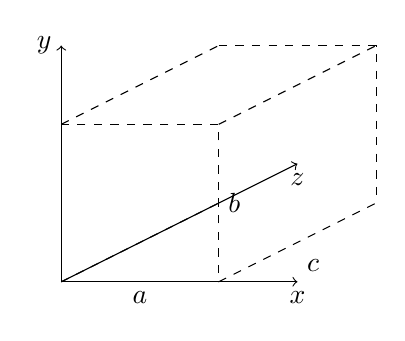
\begin{tikzpicture}
       \draw[dashed] (0,0) -- (2,0) -- (2,2) -- (0,2) -- (0,0); 
       \draw[dashed, thin] (0,0) -- (2,1);
       \draw[dashed, thin] (0,2) -- (2,3);
       \draw[dashed, thin] (2,2) -- (4,3);
       \draw[dashed, thin] (2,0) -- (4,1);
       \draw[dashed, thin] (2,3) -- (4,3) -- (4,1);
       \node[below] at (1,0) {$a$};
       \node[right] at (2,1.0) {$b$};
       \node[right] at (3,0.2) {$c$};
       \draw[->] (0,0) -- (3,0) node[below] {$x$};
       \draw[->] (0,0) -- (0,3) node[left] {$y$};
       \draw[->] (0,0) -- (3,1.5) node[below] {$z$};
    \end{tikzpicture}
    \caption{Overview}
    \label{fig:2022_9}
\end{figure}\noindent
The wavefunction is seperable by nature, so one can write the following, with the natural boundary conditions:
\begin{align*}
    \psi_{n,m,l}(x,y,z) = c\sin\left(\frac{n\pi}{a}x\right)\sin\left(\frac{m\pi}{b}y\right)\sin\left(\frac{l\pi}{c}z\right)
\end{align*}
\vspace*{3cm}
\begin{center}
    \color{red}
    \boxed{\color{black}\text{This summerizes both the previous exam and the compendium}}
\end{center}